\documentclass[17pt]{beamer} %Makes presentation
%\documentclass[handout]{beamer} %Makes Handouts
\usetheme{Singapore} %Gray with fade at top
\useoutertheme[subsection=false]{miniframes} %Supppress subsection in header
\useinnertheme{rectangles} %Itemize/Enumerate boxes
\usecolortheme{seagull} %Color theme
\usecolortheme{rose} %Inner color theme

\definecolor{light-gray}{gray}{0.75}
\definecolor{dark-gray}{gray}{0.55}
\setbeamercolor{item}{fg=light-gray}
\setbeamercolor{enumerate item}{fg=dark-gray}

\setbeamertemplate{navigation symbols}{}
%\setbeamertemplate{mini frames}[default]
%\setbeamercovered{dynamics}
\setbeamerfont*{title}{size=\Large,series=\bfseries}
\setbeamerfont{footnote}{size=\tiny}

%\setbeameroption{notes on second screen} %Dual-Screen Notes
%\setbeameroption{show only notes} %Notes Output

\setbeamertemplate{frametitle}{\vspace{.5em}\bfseries\insertframetitle}
\newcommand{\heading}[1]{\noindent \textbf{#1}\\ \vspace{1em}}

\usepackage{bbding,color,multirow,times,ccaption,tabularx,graphicx,verbatim,booktabs}
\usepackage{colortbl} %Table overlays
\usepackage[english]{babel}
%\usepackage[latin1]{inputenc}
%\usepackage[T1]{fontenc}
\usepackage{lmodern}

%\author[]{Thomas J. Leeper}
\institute[]{
  \inst{}%
  Department of Government\\London School of Economics and Political Science
}

\usepackage{tikz}
\usetikzlibrary{shapes,arrows}

\title{Case Comparisons}

% How do comparisons between cases help us to make inferences about causality? How do we select cases so that comparisons between them are informative about theories and hypotheses?


\date[]{}

\begin{document}

\frame{\titlepage}

\frame{\tableofcontents}

\section[Case Studies]{Case Studies Continued}
\frame{\tableofcontents[currentsection]}

\frame{

\frametitle{What is a case study?}

\begin{itemize}\itemsep0.1em
\item Definition: ``an intensive study of a single unit for the purpose of understanding a larger class of (similar) units'' (Gerring 2004, 342)
\item Broad uses:
	\begin{itemize}
	\item Description
	\item Induction/Theory development
	\item Theory testing
	\item Exploration of mechanisms
	\item Concept definition and measurement
	\end{itemize}
\end{itemize}

}

% not simply attempting to score a case on a variable but attempting to understand it at a very deep level



\frame{

\frametitle{What counts as a case?} % activity

\begin{itemize}\itemsep0.25em
\item<2-> The more important question is what is something a \textit{case of}
\item<2-> Cases are instances of a concept or phenomenon
	\begin{itemize}
	\item<3-> What is the Brexit referendum a case of?
	\item<4-> What is Islamic State a case of?
	\item<5-> What is Angela Merkel a case of?
	\item<6-> What is Sep. 11th a case of?
	\item<7-> What is Wales a case of?
	\end{itemize}
\end{itemize}

}

% common cases: countries, subnational units, persons, political parties, events (e.g., acts of terrorism), revolutions, transitions to democracy, wars, policies, legislatures, elections


% an instance or observation can be a case of many different things
% September 11th might be a case of terrorism, of structural deficiencies in buildings, of airplane hijacking, of airport security, of intelligence failure, of presidential leadership, of the onset of war, of "rallying around the flag", etc.
% to study something as a case, you need to know what it is a case *of*


\frame{

\frametitle{Types of testing}

\small

\begin{itemize}\itemsep1em
\item Hypothesis confirming: ``most likely'' case
\item Hypothesis weakening: ``least likely'' case
\item Hypothesis generating: ``deviant'' cases
\item Concept definition: ``new'' cases
\end{itemize}

}


\section{Case Comparisons}
\frame{\tableofcontents[currentsection]}

\frame{

\frametitle{Doner, Ritchie, Slater (2005)}

In pairs, discuss the following:

\begin{itemize}
\item What is the outcome?
\item What is the theory?
\item What are the cases examined?
\item How are the cases compared?
\end{itemize}

You have 3 minutes.

}


\frame{

\begin{center}
\begin{tikzpicture}
\node[anchor=south west,inner sep=0] at (0,0) {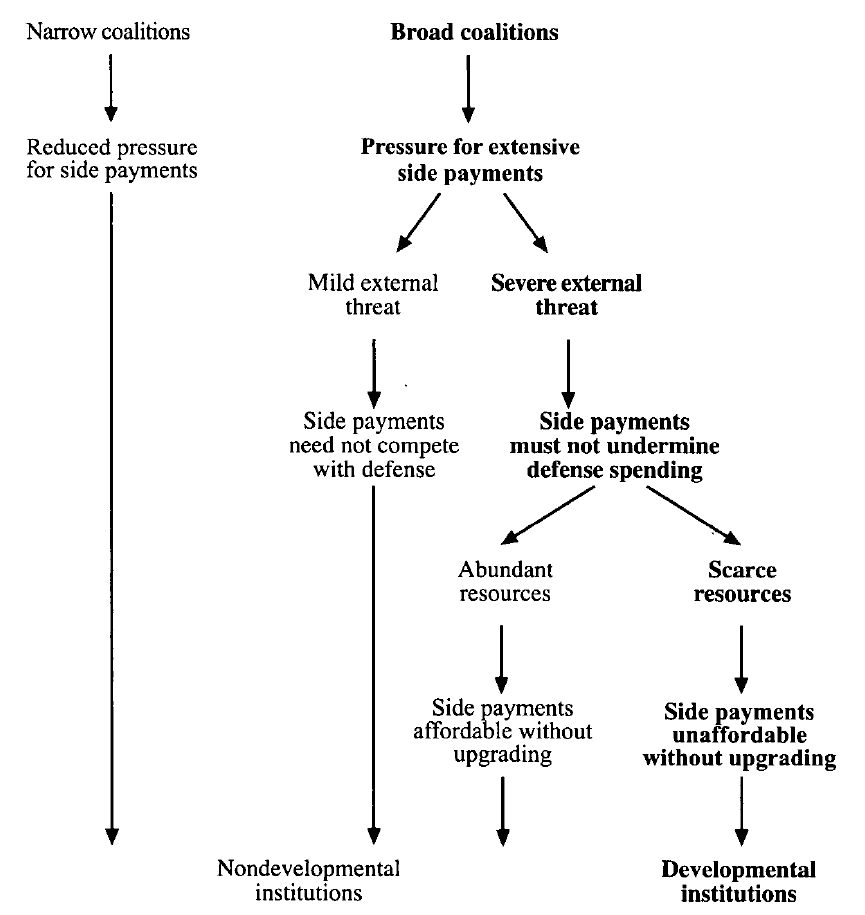
\includegraphics[height=.8\textheight]{images/doner-figure1}};
\draw<2->[red,ultra thick,rounded corners] (0,6.6) rectangle (5,7.25);
\draw<3->[red,ultra thick,rounded corners] (2,4.5) rectangle (5.5,5.25);
\draw<4->[red,ultra thick,rounded corners] (3.5,2.25) rectangle (6.5,3);
\draw<5->[blue,ultra thick,->] (3.7, 6.8) -- (3.7,6) -- (4.5,4.9) -- (4.5,3.7) -- (5.85,2.9) -- (5.85,0.5);
\end{tikzpicture}
\end{center}

{\tiny Figure 1 from Doner, Ritchie, Slater (2005). ``Systemic Vulnerability and the Origins of Developmental States.'' \textit{International Organization} 59: 327--361.\par} 
}


\frame{
\frametitle{Mill's methods\footnote{Discussed in Holland (1986) from Week 2}}

\begin{enumerate}\itemsep0.5em
\item \textbf<2->{Agreement}
\item \textbf<2->{Difference}
\item \textbf<2->{Agreement and Difference}
\item Residue
\item Concomitant variations
\end{enumerate}
}

\frame{

\frametitle{Using Mill's Methods}

\begin{enumerate}\itemsep0.5em
\item<1-> Identify an outcome to explain
\item<2-> Find cases and score on outcome
	\begin{itemize}
	\item Need outcome variation
	\end{itemize}
\item<3-> Categorize cases on possible explanations
	\begin{itemize}
	\item Need variation
	\end{itemize}
\item<4-> Apply Mill's methods to:
	\begin{itemize}
	\item Identify deterministic causes
	\item Eliminate deterministic causes
	\end{itemize}
\end{enumerate}

}

% what is the outcome in Doner et al.?


\frame{
\frametitle{Agreement}

\begin{quote}
If two or more instances of the phenomenon under investigation have only one circumstance in common, the circumstance in which alone all the instances agree, is the cause (or effect) of the given phenomenon.
\end{quote}

Often called ``most different systems'' design.

}


% how do Doner et al. use the method of agreement?
% use this to eliminate potential causes

\frame<1-2>[label=table2]{
\begin{center}
\begin{tikzpicture}
\node[anchor=south west,inner sep=0] at (0,0) {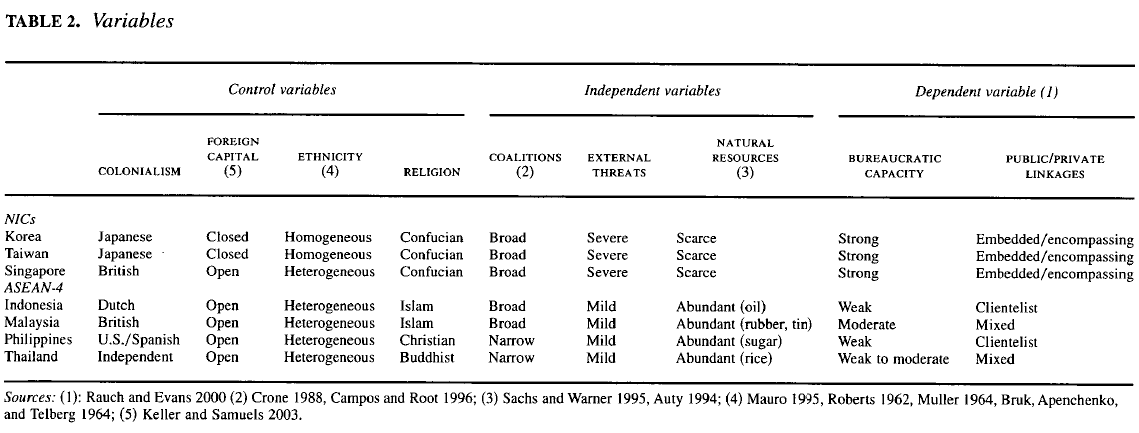
\includegraphics[width=\textwidth, trim={0 0 8cm 0}, clip]{images/doner-table2}};
\draw<2>[red,ultra thick,rounded corners] (1,0.75) rectangle (6.2,4);
\draw<3>[red,ultra thick,rounded corners] (6.2,0.75) rectangle (10.75,4);
\end{tikzpicture}
\end{center}

{\tiny Table 2 from Doner, Ritchie, Slater (2005). ``Systemic Vulnerability and the Origins of Developmental States.'' \textit{International Organization} 59: 327--361.\par} 
}
% table showing method of agreement for Doner et al.



\frame{
\frametitle{Difference}

\small

\begin{quote}
If an instance in which the phenomenon under investigation occurs, and an instance in which it does not occur, have every circumstance save one in common, that one occurring only in the former; the circumstance in which alone the two instances differ, is the effect, or cause, or an necessary part of the cause, of the phenomenon.
\end{quote}

\normalsize 

Often called ``most similar systems'' design.

}

% how do Doner et al. use the method of agreement?
% use this to identify potential causes


\againframe<1,3>{table2}



\frame{
\frametitle{Agreement and Difference}

\small

\begin{quote}
If two or more instances in which the phenomenon occurs have only one circumstance in common, while two or more instances in which it does not occur have nothing in common save the absence of that circumstance; the circumstance in which alone the two sets of instances differ, is the effect, or cause, or a necessary part of the cause, of the phenomenon.
\end{quote}

}


\frame{

\frametitle{{\large Limitations of Mill's Methods}}

\begin{itemize}\itemsep0.5em
\item Necessary causes (Deterministic)
\item Works best with limited number of variables
	\begin{itemize}
	\item Multiple causation is difficult to accommodate
	\end{itemize}
\item Works best with limited number of cases
\item Assume all potential explanations not examined do not matter
\end{itemize}

}

\frame{}



\section[Uses of Case Studies]{Five Uses of Case Studies}
\frame{\tableofcontents[currentsection]}


\frame{
\frametitle{1: Description}
\begin{itemize}\itemsep1em
\item Case study might be descriptive
\item Historical or interpretive
\item Think ``biography''
\end{itemize}
}

% what happened; when did events happen; who was involved; etc.

\frame{
\frametitle{2: Theory development}
\begin{itemize}\itemsep0.5em
\item Case is an instance of a phenomenon
\item There is some outcome to be explained
	\begin{itemize}
	\item Outcome is case itself
	\item Outcome of a case
	\item Outcome as part of case
	\end{itemize}
\item Look for ``Causal Process Observations''
\item Attempt to identify generalizable explanations
\end{itemize}
}

% we see this in the second half of Doner et al.


\frame{
\frametitle{{\large Causal Process Observations}}

\normalsize

\begin{itemize}\itemsep0.5em
\item Definition: ``An insight or piece of data that provides information about the context, process, or mechanism, and that contributes distinctive leverage in causal inference''\footnote{Brady and Collier 2004, p.277}
\item Essentially pieces of evidence that offer insight into within-case counterfactuals
\end{itemize}
}

% more on this next week

\frame{
\frametitle{3: Theory testing}
\begin{itemize}\itemsep1em
\item ``Actual case'' comparisons
	\begin{itemize}
	\item Mill's methods
	\end{itemize}
\item Fearon's ``Counterfactual method''
\item Process tracing
\end{itemize}
}


% thinking counterfactually
	% can we observe the counterfactual (in another case, in the same case at another time, in a collection of other cases)?
	% if not, can we think about what that counterfactual might look like? 
	% see Fearon's use of ``counterfactual method''; thought experiments; hypothetical reasoning
% actual case comparisons need to take the form of Mill's methods

\frame{
\frametitle{4: Mechanisms}
\begin{itemize}\itemsep0.5em
\item Imagine you already have evidence for a causal relationship
\item A case study can help you explore or test for ``mechanisms'' of that effect
\item This is our focus next week
\end{itemize}
}

\frame{
\frametitle{5: Concept Definition}
\begin{itemize}\itemsep0.5em
\item Sometimes you don't know what you are studying
\item Case studies can clarify what something is a \textit{case of}
\item This helps you to:
	\begin{itemize}
	\item Refine your concept definition
	\item Improve measurement
	\end{itemize}
\end{itemize}
}

\frame{}


\frame{

\frametitle{Preview}

\begin{itemize}\itemsep1em
\item Next week: Process-tracing
\item Problem Set 3 Due
\item Start thinking about research topics for Week 11
\end{itemize}

}


\frame{}
% If time is permitting, use TV reality shows as a way to create a typology



\appendix
\frame{}

\end{document}
